\part{Analysis}

A hand digit recognition neural network (HDR-NN) model is implementated in \texttt{C}, \texttt{C++} using Eigen, Python using Numpy, and Pytorch via its \texttt{C++} interface. The performance of HDR-NN training implementations was evaluated on the MCIMX6Q-SDB evaluation board, which was programmed with an Embedded Linux built using the Yocto Project. To gauge the effectiveness of the models, we compared model accuracy, execution time, and peak memory usage while altering the number of layers and neurons in each layer. The results of these measurements are presented in the following chapters along with discussions on the obstacles encountered in developing the neural network model and compiling it to operate on the target hardware.

\subsection*{Benchmark Overview}

HDR-NN is implemented in different paradigms, specifically \texttt{C}, \texttt{C++}, Python, and Pytorch. Each of these applications contain a fully connected feedforward neural network composed of multiple layers of neurons connected in a directed graph. The model has a constant input size of 784 which correspond to the 28 x 28 pixel dimensions of the images of the MNIST dataset. The output size of the network is 10, corresponding to the 10 possible digits that the image contains. The number and size of the hidden layers are configurable in each of the different implementations.

The MNIST dataset was selected to train the model, which contains 60,000 training images and 10,000 test images of hand-written digits. The model is trained using stochastic gradient descent, which is an optimization algorithm used to minimize a loss function. The backpropagation algorithm is used to calculate the gradients of the loss function with respect to the weights of the network. Finally, the mean square error loss function is used to measure the difference between the predicted output and the actual output of the network. The values of the biases and weights are initialized randomly with the PNGR random generator and a starting seed which are chosen to be identical for the different benchmark applications. The training hyperparameters for the benchmark runs are set to 1 epoch with a batch size of 10, a learning rate of 3, with the network using the sigmoid activation function.

It is essential that the hardware utilzed for benchmarking closely resemble the i.MX6 processor on Scania ECUs, as this will make it easier to replicate the experiment on a repurposed ECU and will also provide the most precise results. The MCIMX6Q-SDB evaluation board, which is armed with four 32-bit Cortex A9 cores, is an ideal choice. The Cortex A9 core is equipped with ARM V7 instruction set architecture and a powerful VFPv3 floating point unit with NEON SIMD capabilities. The processor has 32 KB instruction and data L1 caches, 1 MB L2 cache and 1 GB DDR3 SDRAM memory. The benchmark applications are designed to be run on a single core of the i.MX6 processor, although it supports quad-core, to ensure the experiment is straightforward and easier to manage. This will also guarantee that the results are precise and accurate.

The yocto project is used to create a custom embedded linux distribution for the \texttt{imx6qsabresd} machine. The NXP yocto project guide \cite{nxp-yocto} provides the instructions for building the Linux image, and additional packages such as cmake, python3 are installed during the build. The resulting image file, which used to flash the hardware, has a size of $\sim$ 300Mb.

The accuracy of the model is evaluated after each training epoch on the MNIST test set. After the training of the model for 30 epochs, the final weights and biases of the network and the accuracy on the test set are saved for analysis. This data is used to verify the correctness of the neural network model in each benchmark application.

The GNU time program is a great tool for monitoring the performance of applications. It allows us to measure the execution time and peak memory usage, which is used to compare the effectiveness of training the neural network model on the custom hardware implemented with different paradigms.

A python script was developed to run the experiment, executing each of the benchmark applications (\texttt{C}, \texttt{C++}, Python, Pytorch) one after the other. Every benchmark application is designed to be repeated 10 times, and all the measurements for each of the hidden layer configurations are saved for each of these iterations. The average values of the model accuracy, execution time and peak memory usage across all iterations are utilized for the analysis.

% ============================================
%        Measurement
% ============================================

\chapter{Measurement}

The benchmark applications were executed on an embedded linux operating system and the measurements were taken primarily based on the \textit{times} system call and \texttt{perf\_events} linux API. The primary tools for current measurement values given in the following chapter were taken using the GNU time. GNU Time provides timing statistics such as the elapsed real time between invocation and termination, the user CPU time, and the system CPU time, the later two via the \textit{times} system call API. GNU Time also provides additional information on other resource usage such as the memory, I/O, and IPC calls where available.

The priliminary measurements for the different executions completed with different learning algorithm parameters and model shapes across implementations were timing statistics and maximum resident set size (alternatively refered to as peak memory utilisation in the following chapter)

\section{Benchmark Application Parameters}

The benchmark applications all had the same configurable parameters for their learning algorithm and network structure. Initial testing of the different benchmark applications were completed seperately with different configurations. These test runs were used to come up with estimates as to how long each run of the training sequence with the different parameters would take and then used to come up with the network shape sizes, and other learning algorithm parameters.

Initially, the network's single hidden layer shape was varied according to powers of two, with the \texttt{C} and \texttt{C++} variants tested with 2, 4, 8, 32, 128, 256, 512, 1024 and so on before adding another hidden layer. The additional hidden layer varied sizes from (16, 16), to (32, 16) and (16, 32), then (128, 16), etc. The final list of shapes and their corresponding shapes for which the measurements results are state in the next chapter are shown in the following table.

\begin{table}[ht]
	\centering
	\begin{tabular}{ |p{11em}|p{14em}| }
		\hline
			\textbf{Hidden layer shape} & \textbf{HDR-NN parameters} (total)\\
		\hline
			2 & 1600 \\
		\hline
			4 & 3190 \\
		\hline
			8 & 6370 \\
		\hline
			16,16 & 13002 \\
		\hline
			32 & 25450 \\
		\hline
			48,48 & 40522 \\
		\hline
			64,16 & 51450 \\
		\hline
			72 & 57250 \\
		\hline
			82,36,16 & 68120 \\
		\hline
			96,96 & 85642 \\
		\hline
			104 & 82690 \\
		\hline
			114 & 90640 \\
		\hline
			128 & 101770 \\
		\hline
	\end{tabular}
\end{table}

The \hyperref[section:hdrnn-ux]{section on UX} in the Design chapter describes how the shape and epochs parameters were configured.

\section{Compilation Options}

All the compiled benchmark programs used the GCC compiler and its \texttt{-O2} optimisation flag. Several other optimisation possibilities were possible and tried out however the data present for \texttt{-O2} was fixed for all the applications for uniformity.

The general suite of compiler optimisations from GCC 11.3 are clever enough to use SIMD, inlining, strength reduction, and a suite of powerful optimisations.

\section{Profiling Analysis}

A \texttt{perf\_events} based record was conducted using the \texttt{perf} utility for all the programs. Flame graphs were generated for the same as shown attached below revealing the areas where the applications were spending the most time on.

\begin{figure}[ht]
	\centering
	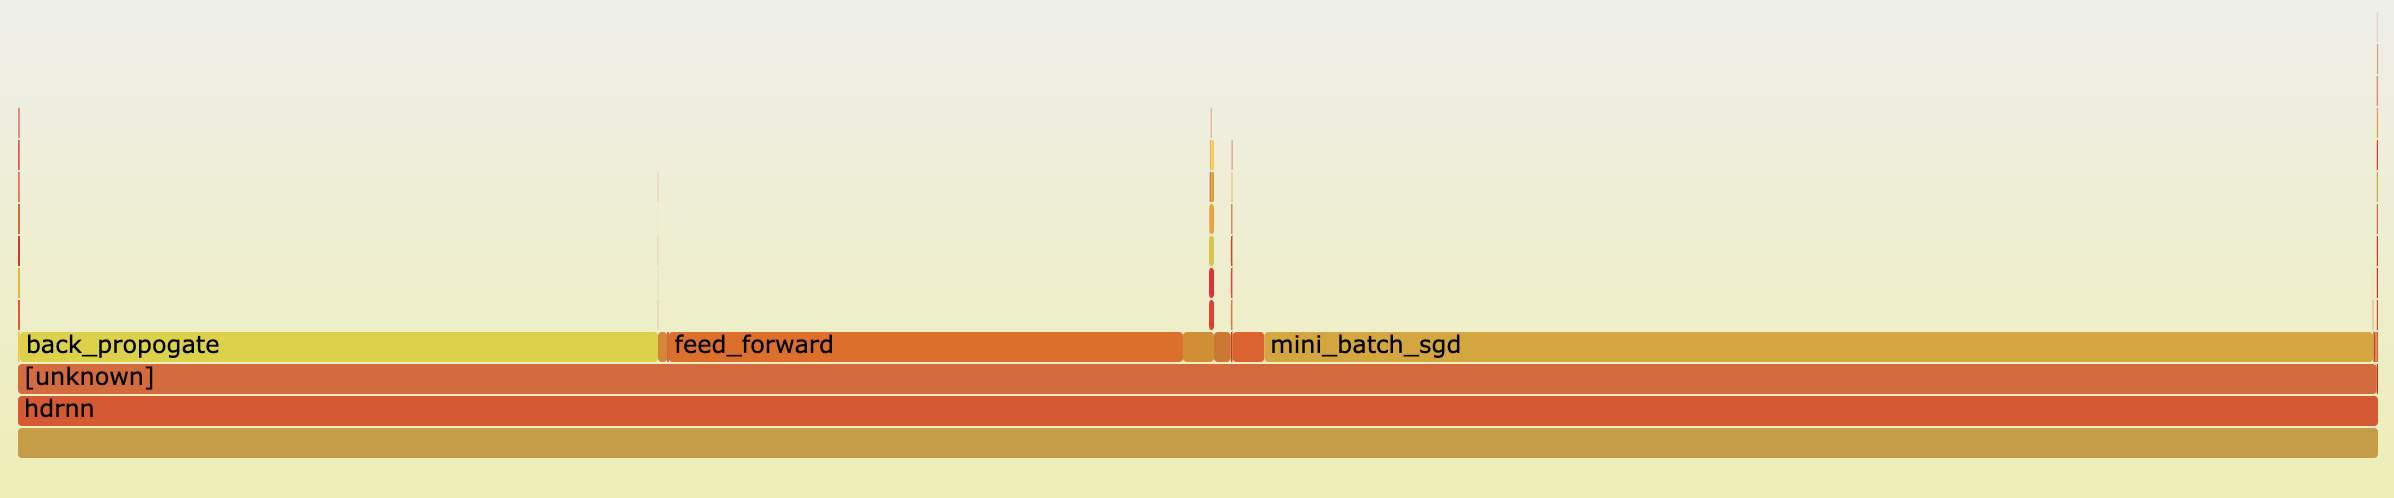
\includegraphics[scale=0.34]{c-math.h-fg.png}
	\caption{c-math.h}
\end{figure}

\begin{figure}[ht]
	\centering
	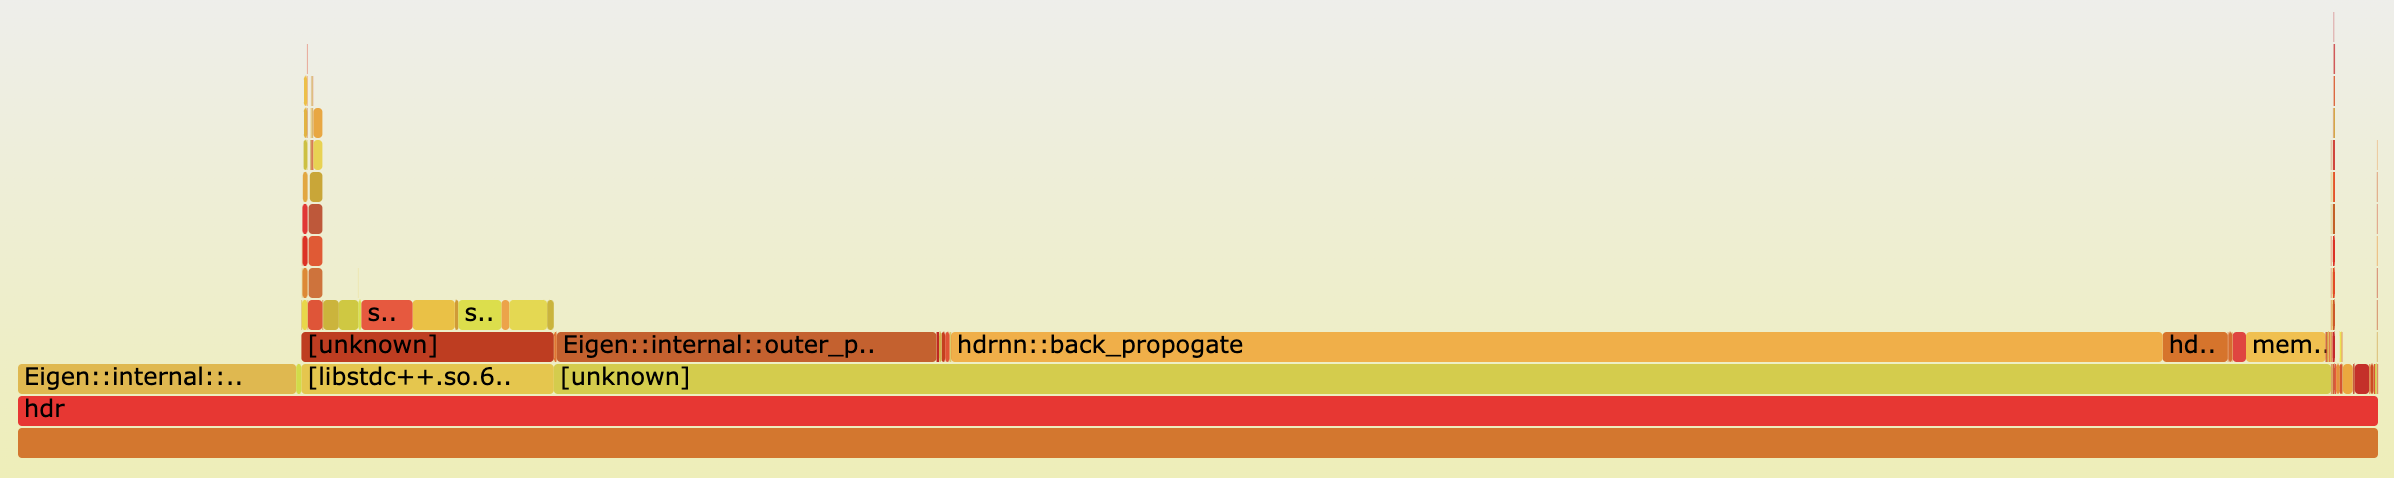
\includegraphics[scale=0.34]{cpp-eigen-fg.png}
	\caption{cpp-eigen}
\end{figure}

\begin{figure}[ht]
	\centering
	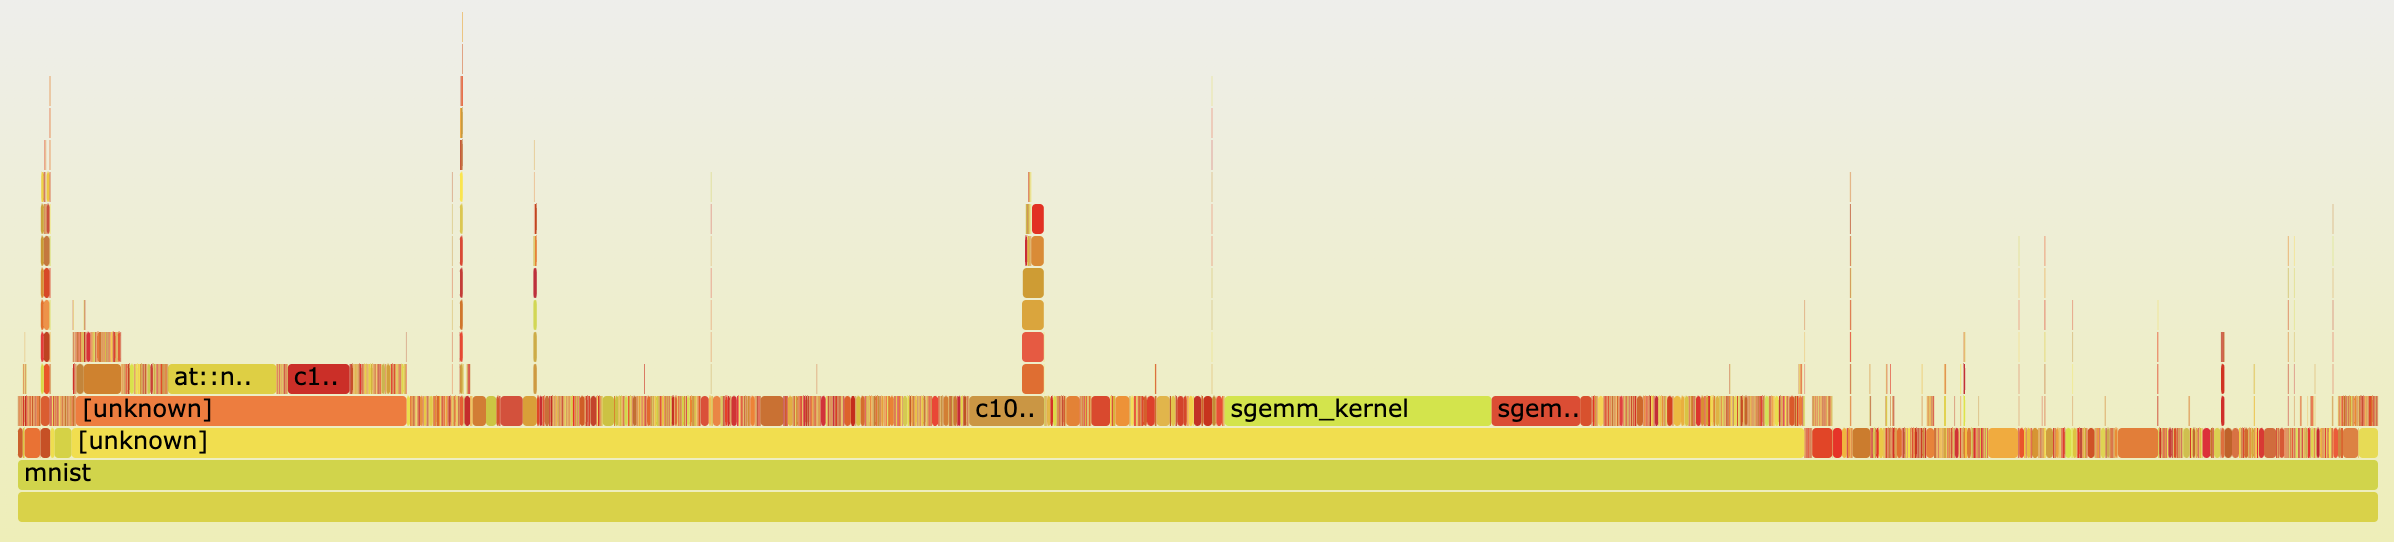
\includegraphics[scale=0.34]{cpp-libtorch-fg.png}
	\caption{cpp-libtorch}
\end{figure}

\begin{figure}[ht]
	\centering
	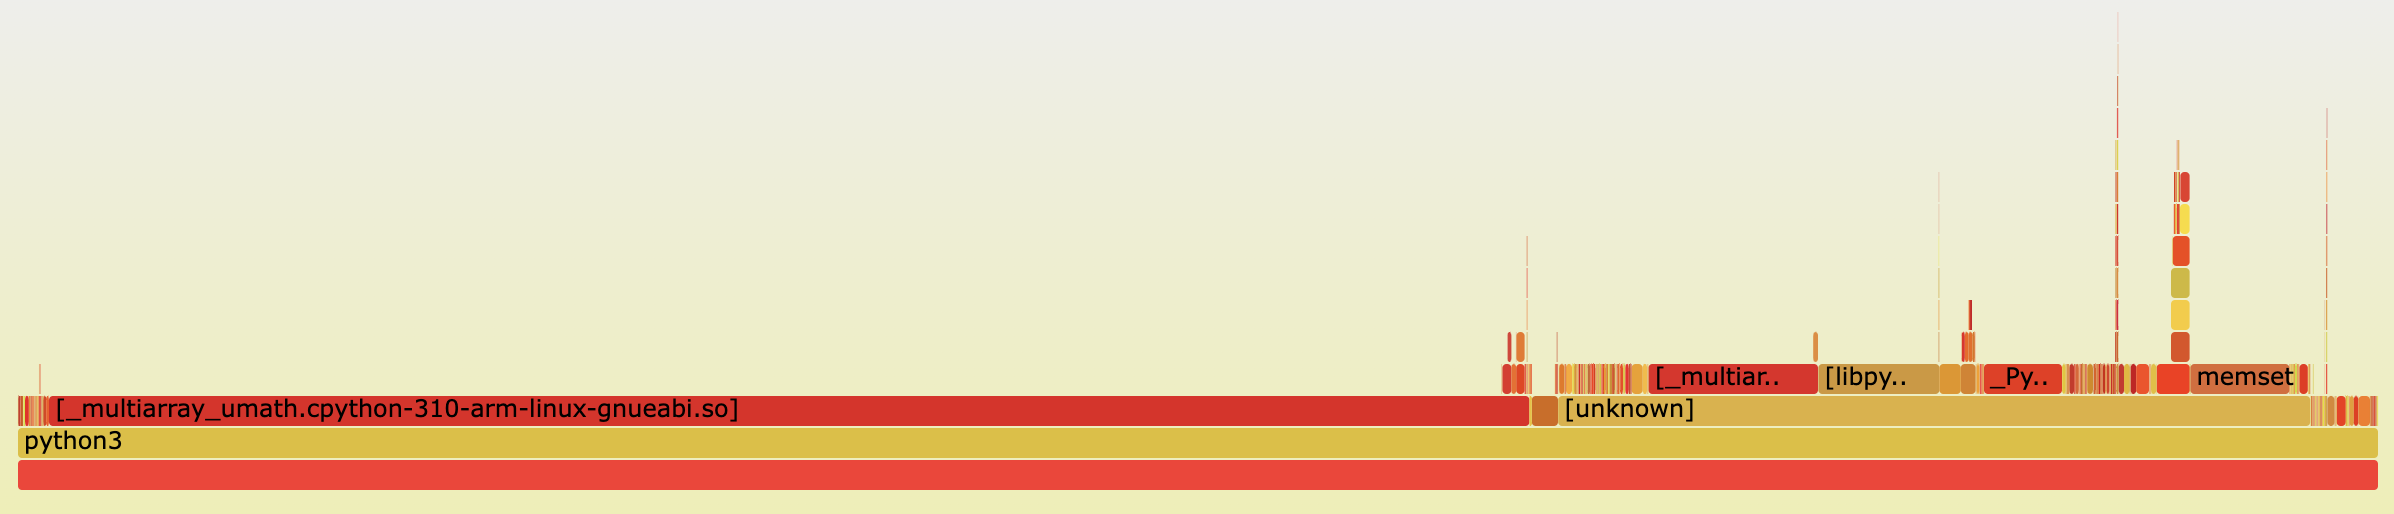
\includegraphics[scale=0.34]{python-numpy-fg.png}
	\caption{python-numpy}
\end{figure}

\subsection{Memory Profile}

Heaptrack is an alternative to the popular valgrind programming tool for memory profiling that comes under the KDE gear of applications by the KDE community. Heaptrack was used to profile the memory of the benchmark application programs under execution

\begin{figure}[ht]
	\centering
	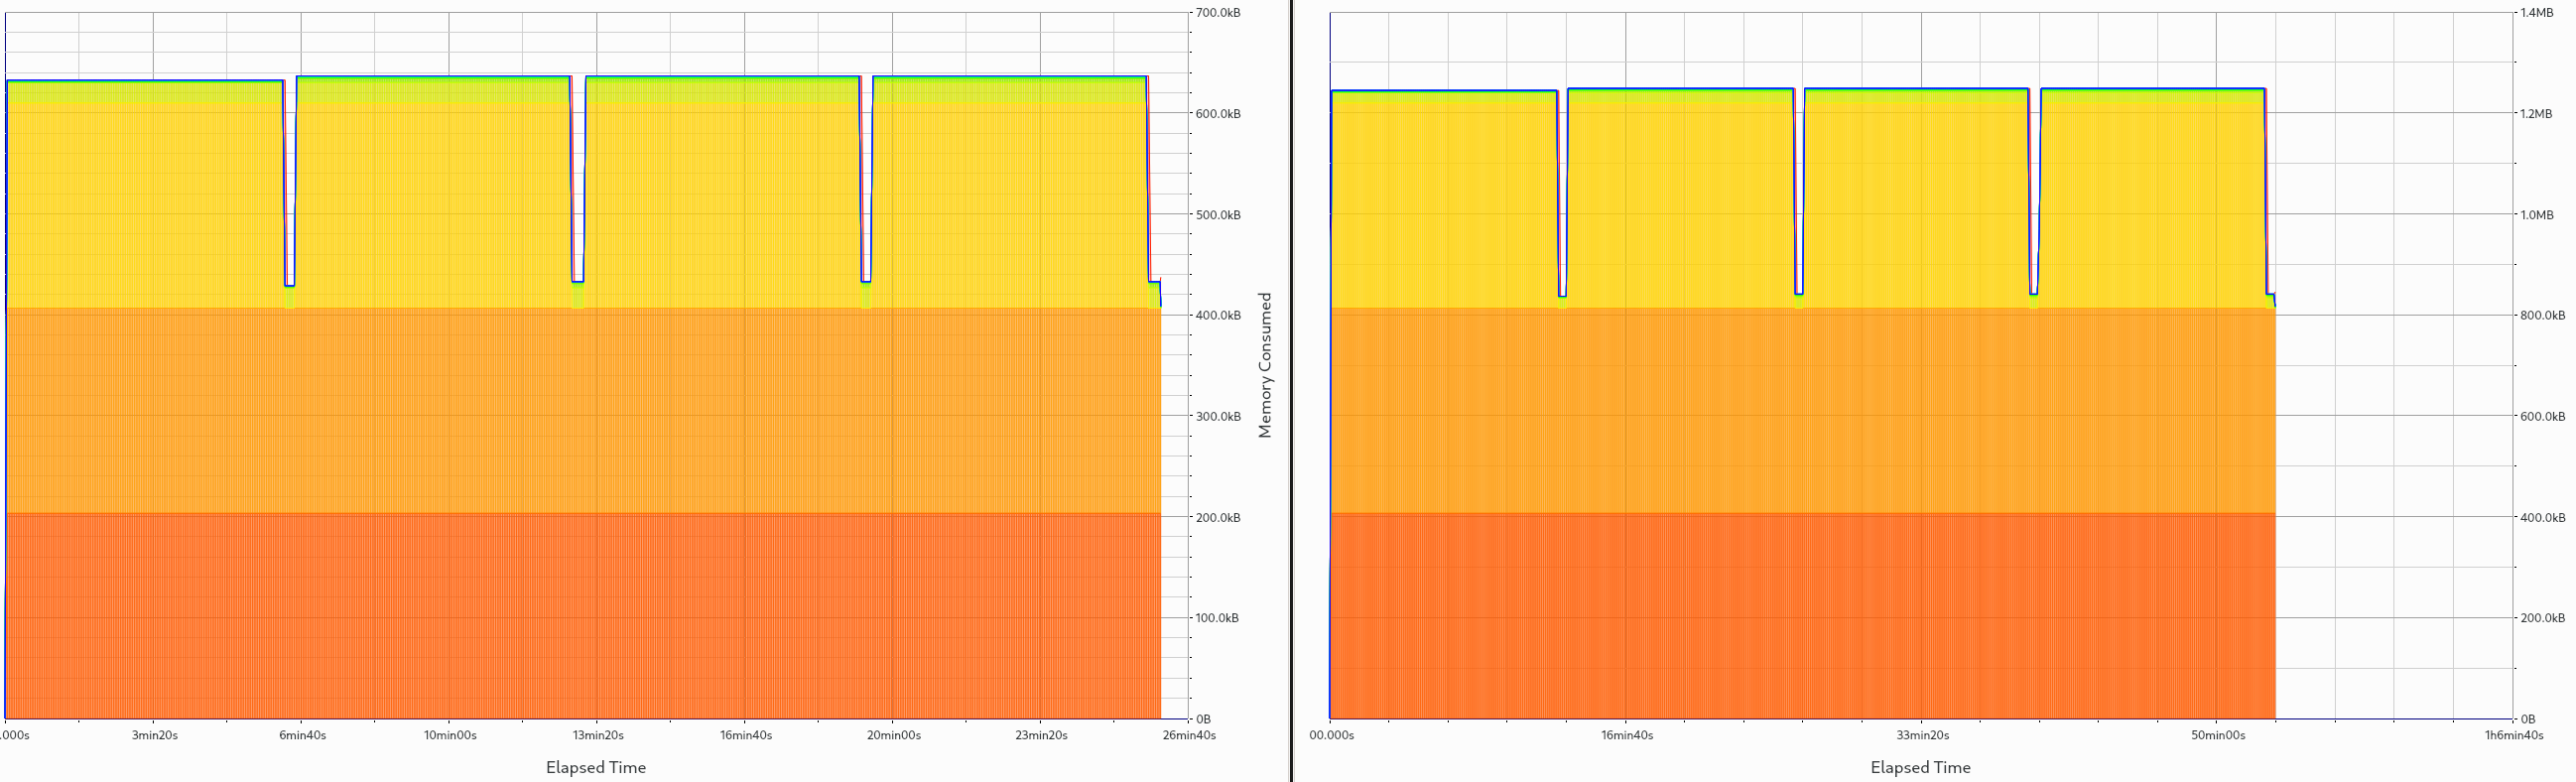
\includegraphics[scale=0.15]{heaptrack-compare.png}
	\caption{c-math.h with 2 different shapes}
\end{figure}

\begin{figure}[ht]
	\centering
	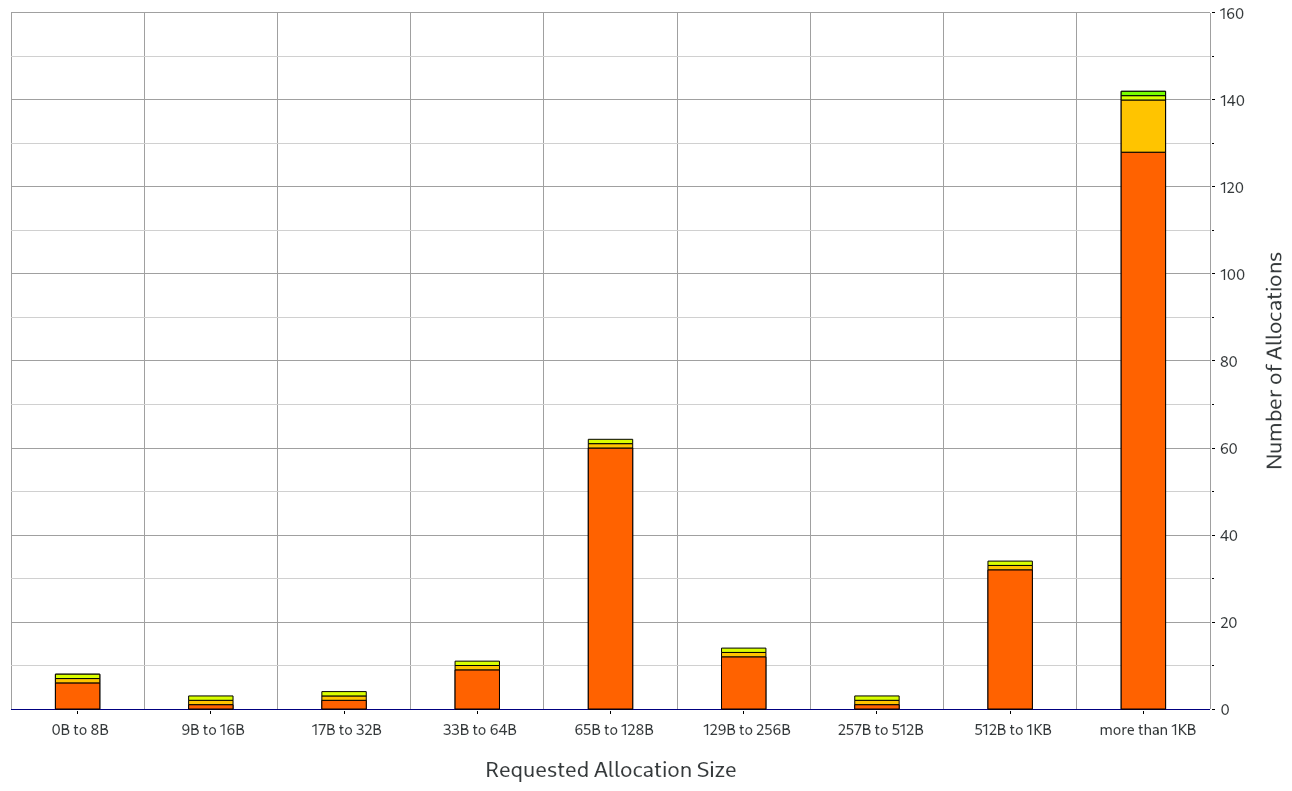
\includegraphics[scale=0.32]{c-math.h-allocations.png}
	\caption{c-math.h allocations}
\end{figure}

% ============================================
%        Results
% ============================================

\chapter{Results}

This chapter presents the results of the benchmark application runs. The first section contains a brief look at the analysis on the neural network accuracies for the different implementations. The second section considers the performance of the benchmark applications followed by the third section that details their differences.

% TODO : Include a paragraph regarding the reliability of the measurements (coefficient of variation of the multiple measurements, assess the degree of variability among the various trials, the mean and standard deviation were calculated across all runs, and their ratioes indicating the level of variation between different tests)

\section{Evaluating Correctness}

As the benchmark applications are developed to be identical by keeping the same structure and configurations, the model accuracy is expected to be similar. Figure \ref{hdrnn-accuracy} showcases that the different implementations perform similarly irrespective of the number of parameters.

% TODO : Remove a few bars from the accuracy plot to make it more readable

\begin{figure}[!ht]
	\centering
	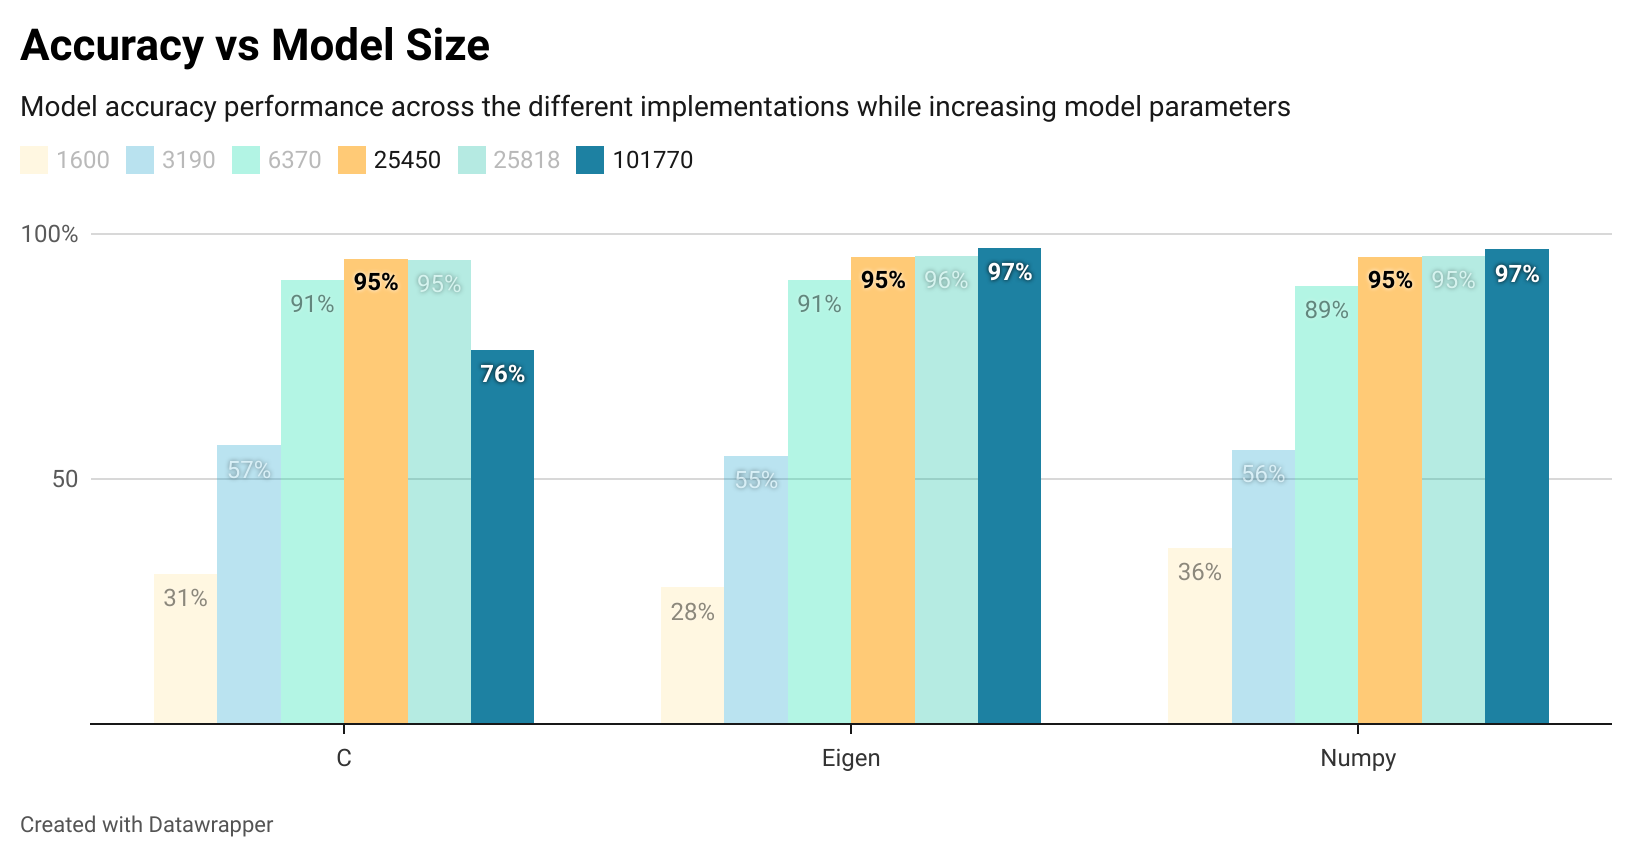
\includegraphics[scale=0.39]{accuracy}
	\caption[HDR-NN Accuracy]{Comparing the accuracy of the different HDR-NN implementations.}
	\label{hdrnn-accuracy}
\end{figure}

Further, an abnormal behaviour can be observed when the number of parameters exceeds 101770. The accuracy of the \texttt{C} implementation decreases due to (an unknown bug).

% \subsection{Weights and Biases}

% TODO : Evaluate the mean squared error in the generated weights and biases between the different implementation.

\section{Evaluating effectiveness}

The primary measures used to evaluate the program performance was execution time and memory utlisation while the applications completed their neural network training.

\subsection{Execution Time}
The training time of the neural network applications increases exponentially as the network size increases by the power of 2 because the number of parameters in a fully connected network increases exponentially as the number of neurons increases. This leads to an increase in the amount of calculations needed for the network to learn, resulting in a longer run time for the training process. This behaviour can be observeed in Figure \ref{hdrnn-exectime} where the execution time increases drastically as number of parameters increases.

\begin{figure}[!ht]
	\centering
	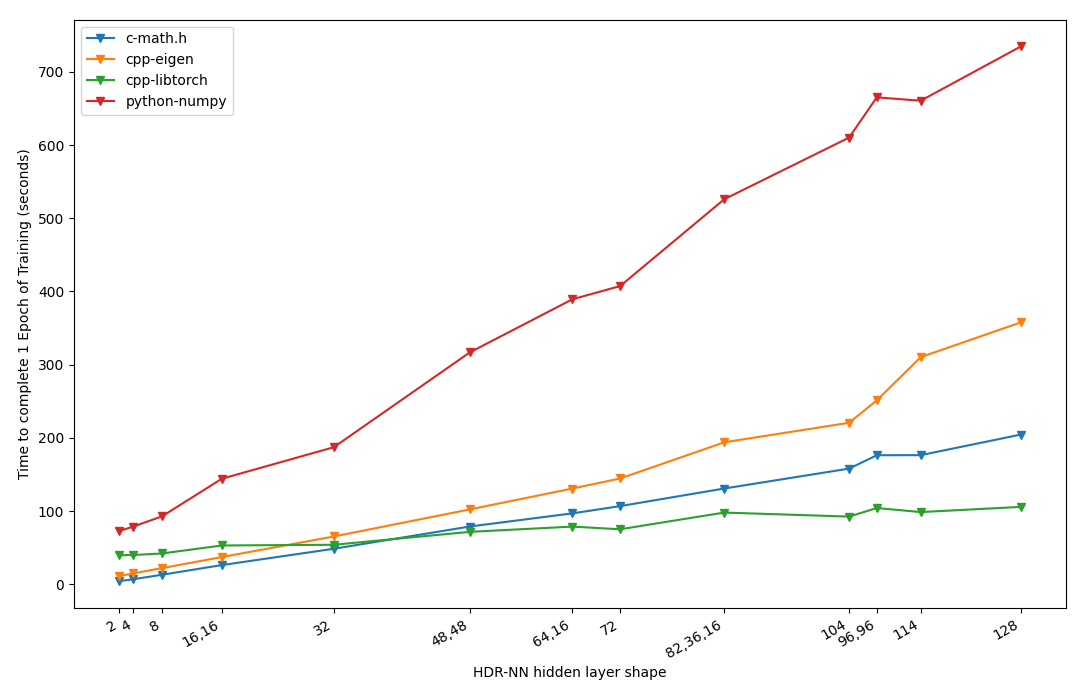
\includegraphics[scale=0.52]{exec-time}
	\caption[Execution Time vs Model Parameters]{Comparing total run time for training the different HDR-NN programs}
	\label{hdrnn-exectime}
\end{figure}

\subsection{Peak Memory Usage}
Regardless of the hidden layer sizes, the peak memory utilisation remains constant for the neural network application across all implementations. The \texttt{C++}, Eigen implementation has the lowest run time memory footprint, while Python Numpy is the least efficient.

\begin{figure}[!ht]
	\centering
	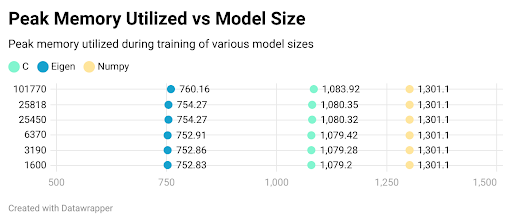
\includegraphics[scale=0.32]{memory-bar}
	\caption[Peak Memory Utilisation]{Peak Memory Utilized during training with different model sizes remain similar within the same implementation}
\end{figure}

Note that the device RAM is 1024 MB however the peak memory utilisation for both \texttt{C} and Numpy are higher than this value. This can be explained by over allocation of memory by the operating system utilising the swap space. The peak memory utilisation measure is using the Maximum resident set size measure, which is roughly the total amount of physical memory assigned to a process at a given point in time. It does not count pages that have been swapped out, or that are mapped from a file but not currently loaded into physical memory.

\subsection{Early stopping}

The training for all the implementations were executed by configuring the number of epochs as 30. This leads to the accuracy of model dropping significantly due to overfitting, which could be avoided if early stopping was implemented. But, early stopping is not implemented as the performance would be completely different and there wouldn't be a standard setting to compare the implementations and the different network model shapes within the same implementations.

\section{Comparing the implementations}

\begin{figure}[!ht]
	\centering
	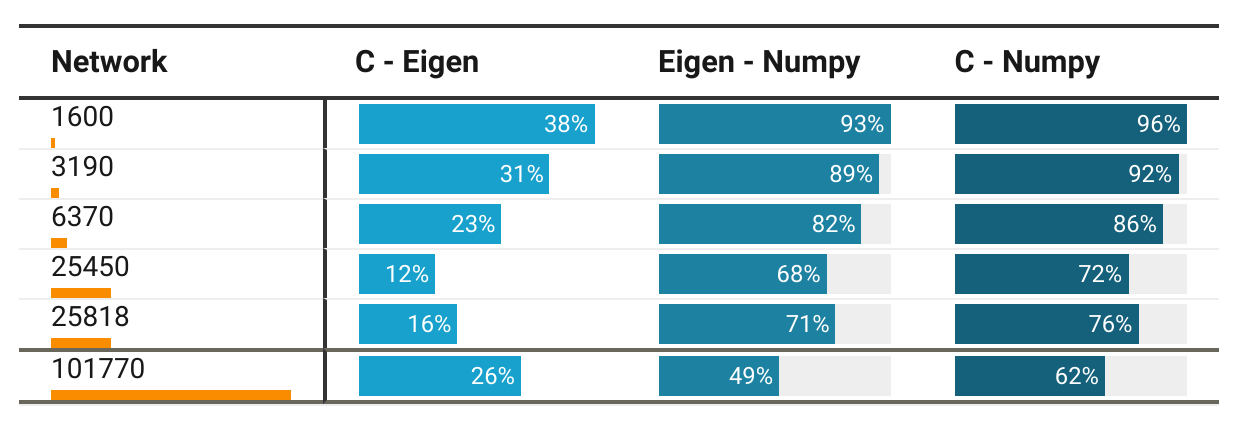
\includegraphics[scale=0.40]{exec_time_comparisons}
	\caption[Execution Time vs Model Parameters]{Percentage difference between the implementations. Example: C is 38\% faster than Eigen for the network size of 1600.}
\end{figure}

\begin{figure}[ht]
	\centering
	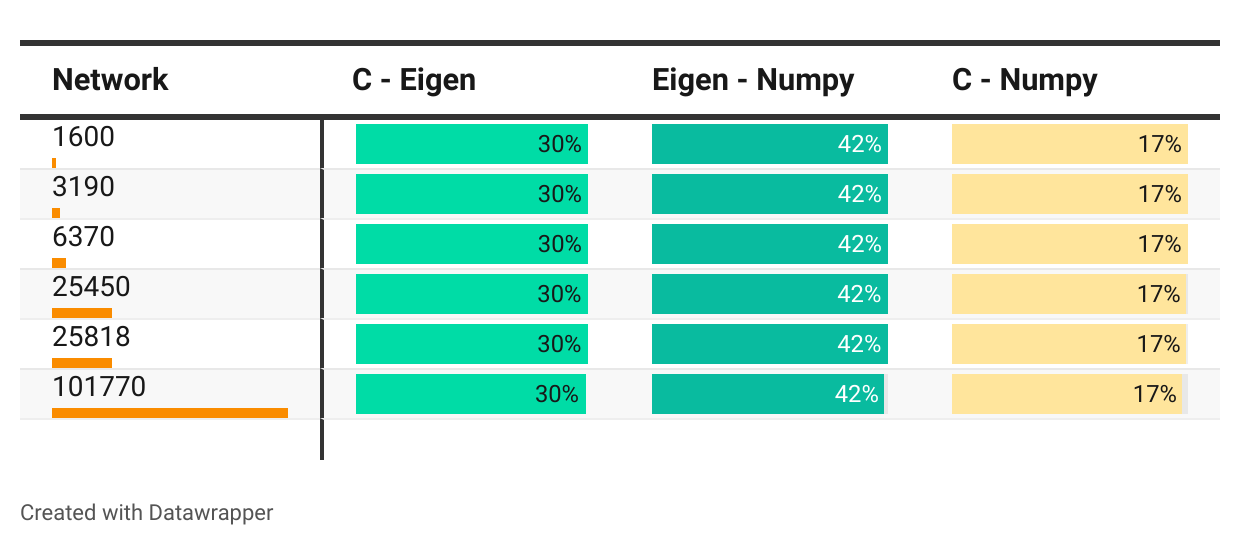
\includegraphics[scale=0.30]{peak_memory_comparisons}
	\caption[Peak Memory Utilisation]{Percentage difference between the implementations}
\end{figure}

The tables in (figure 6.4 and figure 6.5) shows the comparison between C-Eigen, Eigen-Numpy and C-Numpy. It is calculated as the percentage of 1 - (x/y) where x is performance value of the application which has lower value and y is performance value of the application that has higher number.

\subsection{C vs Eigen}
For smaller models, it can be observed that \texttt{C} is faster than Eigen (for the network size of 1600, \texttt{C} is 38 percent faster than Eigen). But as model becomes complex, Eigen perform better and the difference is execution time is less than 15 percent. Again the abnormal behaviour can be observed in case of network size 101770 where \texttt{C} is 26 percent faster than Eigen. More test on the \texttt{C} implementation needs to conducted to identify the bug causing this behaviour.

With regards to memory utilisation Eigen perform better than \texttt{C} by 30\%.

\subsection{C vs Numpy}
\texttt{C} constantly performs much better than Numpy. For the network size 101770, \texttt{C} is 62\% faster.
Numpy utilises 17\% more runtime memory than C.

\subsection{Eigen vs Numpy}
Similar to \texttt{C}, irrespective of network size, Eigen is faster than Numpy by similar margins.

Eigen is efficient in memory utilisation and 42\% better than Numpy.

% ============================================
%        Discussion
% ============================================

\chapter{Discussion}

This chapter contains discussions on the experience while working on the project with the first section examining the process of developing the benchmark applications. The last section describes in brief the distribution of work on the project between the two authors.

\section{Developer Experience}

Embedded environments are greatly varied and working on these platforms are different compared to the more general platforms with comparably reduced support. The greatest challenge in writing the benchmark applications were in sourcing the binaries for the general purpose neural network frameworks. Both Tensorflow and PyTorch do not target the ARMv7 environment that was the primary target for this project. There were are older community tensorflow binaries that are available for the platform that are currently unmaintained, at the time of writing this report. Finally the PyTorch source code was successfully compiled for our target environment using QEMU user-mode emulation.

The embedded hardware and software ecosystems are greatly varied and fragmented leading to less support from the machine learning software ecosystem. The embedded machine learning communities largely contain sprawling technologies that have several different components that have varying degrees of maintanance and create complicated inter relationships over time that are difficult or unwieldy to maintain. This has lead to a lack of good software infrastructure that can support multi-hardware, mult-architecture neural network frameworks.

\subsection{Reverse Engineering Scania C300}

Scania ECU is like a black box with no information. A custom encased hardware that supports ethernet over modem and an UART interface along with hardware circuit schematic document was the only information available regarding the ECU. There is no information regarding the processor,  memory support, bootloader. As the ECU is a production unit, there is no development tools on device and no support to port packages and application to the ECU. Many features on the bootloader, kernel were disabled making it futile to execute the common commands that provide system information.

The task of repurposing the Scania ECU comprised of reverse engineering and obtaining the required hardware/software information and flashing a custom operating system to benchmark the neural network applications. The first task was partially successfully as hardware information such as processor, architecture, I/O interfaces, device tree and software information such as kernel, compiler, glic and versions was obtained. But information regarding the memory layout and boot flow could not be concretely reverse engineered. The second task was not achieved as flashing custom embedded linux always resulted in the ECU being bricked. Experiments conducted from booting the normal operation and from serial download mode had different issues and failed. While flashing from the normal boot, only the bootloader is replaced in the mtd partition. This could have failed because of incorrect u-boot image with wrong device trees or loading kernel failed as version mismatch between bootloader and kernel or checksum failure or size of the file is big overwriting a different region with crucial data. Serial download mode flashing required some crucial information regarding the memory load address and entry point for bootloader, kernel, root file system which is configured in the custom device tree. This information could be obtained from reverse engineering.

\hyperref[rtc-c300]{Appendix II} contains a summary of the efforts involved in reverse engineering the C300 hardware. The project focus shifted to the MCIMX6Q-SDB board after having spend considerable time on the C300.

\section{General Distribution of Work}

The reverse engineering efforts were done in unison between the authors by suggesting then attempting different ideas, with Deepak Venkataram working on soldering and other physical manipulations on the Scania C300. The programming of the benchmark applications was completed by Prasanth Thomas Shaji while the testing of these applications on the MCIMX6Q-SDB were completed by Deepak Venkataram. The primary responsibilities of most activities were divided between the authors however they were performed in concert were possible. The benchmark applications and the report were version controlled in two seperate repositories containing commits from both authors and provides the primary accounting of the distribution of work.

\chapter{Conclusion and Future Work}

Developing of neural network implementations for the embedded environment is considerably more challenging than a traditional general purpose personal computer or server computers. The lack of support of on these platforms for the traditional machine learning frameworks stems from the fragmented nature of the embedded ecosystem. There are several challenges in the way for developing a machine learning framework for embedded devices. The current mature frameworks have some means of providing inference passes on embedded platforms however training on-board is still limited to larger platforms.

The development and testing of the benchmark application HDR-NN revealed the difficulties in targetting the \texttt{armv7hl} architecture. The performance of the benchmark applications showed that PyTorch had considerably higher performance than expected for larger shapes than the hand made \texttt{C} implementation. This could however change by working on performance engineering of the \texttt{C} implementations. However leveraging tool support for performance engineering on these systems are still difficult and requires heavy investment in time.

\section{Future Work}

The initial mandate on the project was to repurpose the Scania C300 to provide a means of targetting the platform reliably. There are yet more technical hurdles to achieving that goal. On-Board Training of neural network models is an active area of reach in TinyML with several efforts in both academia and industry to achieve efficient training algorithms.

\subsection{Porting to C300}

Repurposing the Scania ECU is a technical challenge that was left incomplete during the project. The experience as detailed in \hyperref[rtc-c300]{Appendix II} and through out the report. The attempt concluded without having ported the embedded linux onto the board. Further information on the device tree layout may be extracted by leveraging the \texttt{/proc/device-tree} linux interface and a binary disassembly of the bootloader on-board the device could reveal more information about the memory layout. These efforts were dropped in favour of continuing the work on the MCIMX6Q-SDB.

\subsection{TinyML research on On-Device Training}

Multi-framework and multi-architecture based software infrastructure that allows are being developed my the community in parts such as Modular \cite{mojo}, EdgeImpulse, etc. There are innovative approaches to bring down the memory requirements of deep learning neural network models such as TinyTL \cite{cai2021tinytl} by changing the learning algorithm that will be running on-board.
